\documentclass{article}
\usepackage{graphicx}

\title{Obs. Enquiry - Adrenaline and Adaptation}

\author{Joshua Turcotti}

\begin{document}
\maketitle

I am an avid road and mountain biker, and I lived in New York City during the entire Summer and Fall of 2020. I frequently biked laps of 6 mile paved loop in Central Park, Manhattan, and the extensive dirt trail network in Cunningham Park, Queens. Google-sources images of both locations are on the next page as Figures \ref{CPLoop} and \ref{CHPLoop} respectively. Both activities would always exceed an hour in duration. I will begin by noting a phenomeon specific to the latter, however.

I noticed that during my most intense Cunningham Park rides, after sustaining motion for at least 20 minutes and then coming to a stop and resting, I would experience massive visual disorientation. Specifically, the leaves of the thick foliage overhead would appear to be ``swimming'' and receding away from the focal point of my vision. This would last roughly a minute even under sustained and focussed observation of the foliage. This effect was notable to me in two key ways: 1) Unlike most optical illusions seen in class - it persisted more than a few seconds, and despite all attempts to concentrate it did not desist; 2) Attempts to reproduce every aspect failed unless extreme Adrenaline was part of the attempt. I will now elaborate on the 2nd peculiarity.

First, I will describe my two varities of attempts at reproduction. The former ooccured in Manhattan's Central Park. These rides would involve 18-24 miles of sustained speeds in the mean range 25-35mph, and heavy exertion. The path was substantially wider and more regular than the trails in Cunningham park (once again see figures \ref{CPLoop} and \ref{CHPLoop}), still surrounded by thick foliage in the summer months I am describing. I did not percieve any variety of the swimming and receding effect noted above after these rides. The second attempt at reproduction consitutes rides at Cunningham Park of identical length (mean 20 min bursts), time of year, and mean speed (5-15mph), but on trails rated as less difficult. This rating means that they featured fewer surprsing technical features such as jumps, drops, and rock gardens (an example of the latter is pictured in Figure \ref{RockG}). On such attempts, the swimming and receding effect was not observed. My tentative conclusion is that the apaptation effect witnessed in the foliage was heavily exacerbated by adrenaline. I believe that my variety of attempts are sufficient to conclude that factors such as activity duration, activity setting, and activity speed did not play a role. In general, I hypothesize that the human brain relies more heavily on heuristics and is more inclined to perform perceptory adaptation during the ``Flight-or-Fight'' response of dangerous activities such as technical mountain biking. 

\begin{figure}[p]
  \caption{Central Park Loop - Typical Portion}
  \label{CPLoop}
\centering
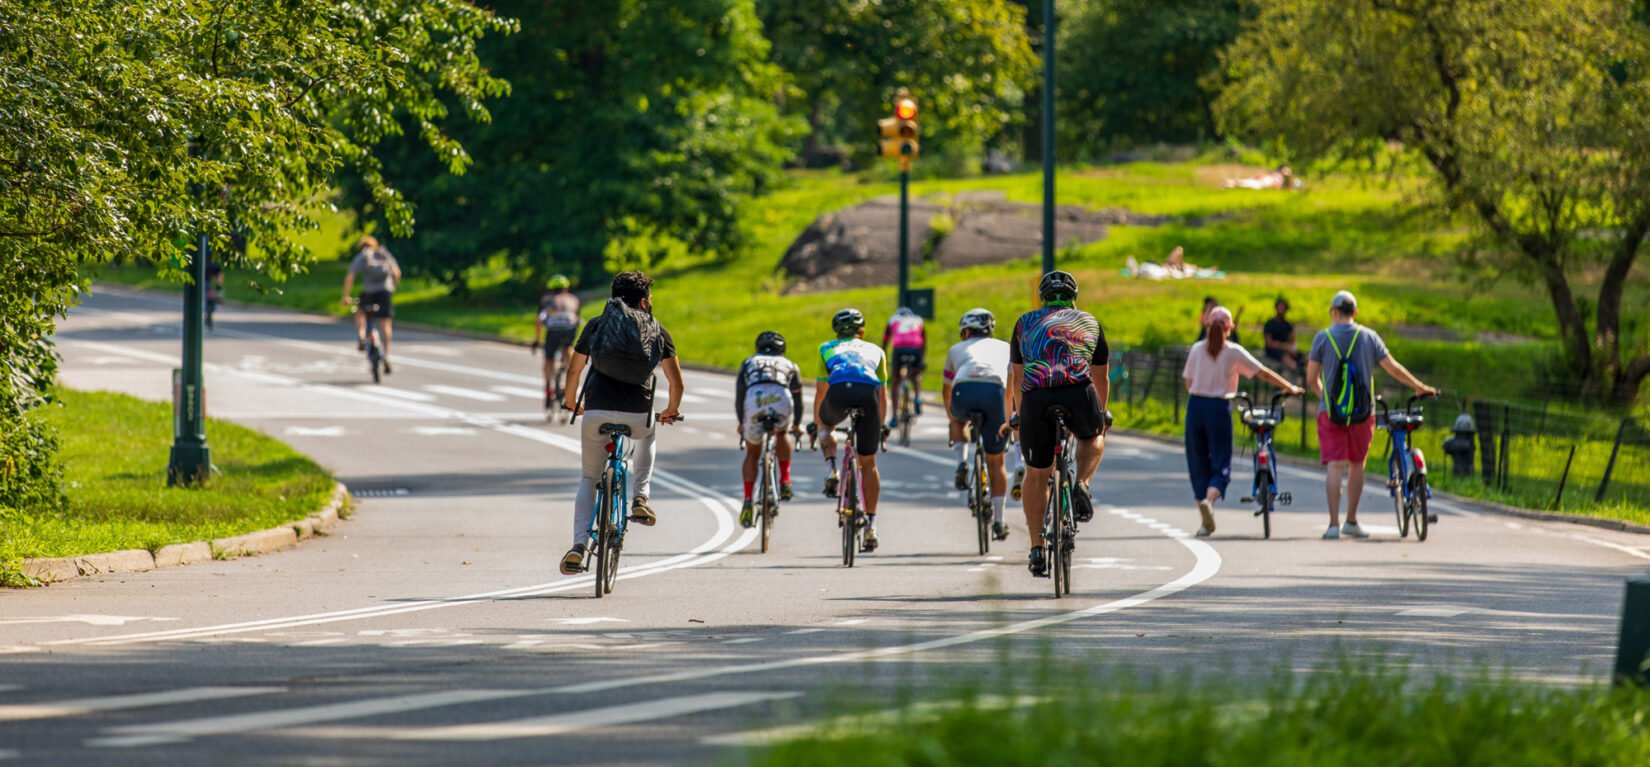
\includegraphics[width=0.75\textwidth]{ManhattanLoop.jpg}
\end{figure}

\begin{figure}[p]
  \caption{Cunningham Park - Typical Trail Segment}
  \label{CHPLoop}
\centering
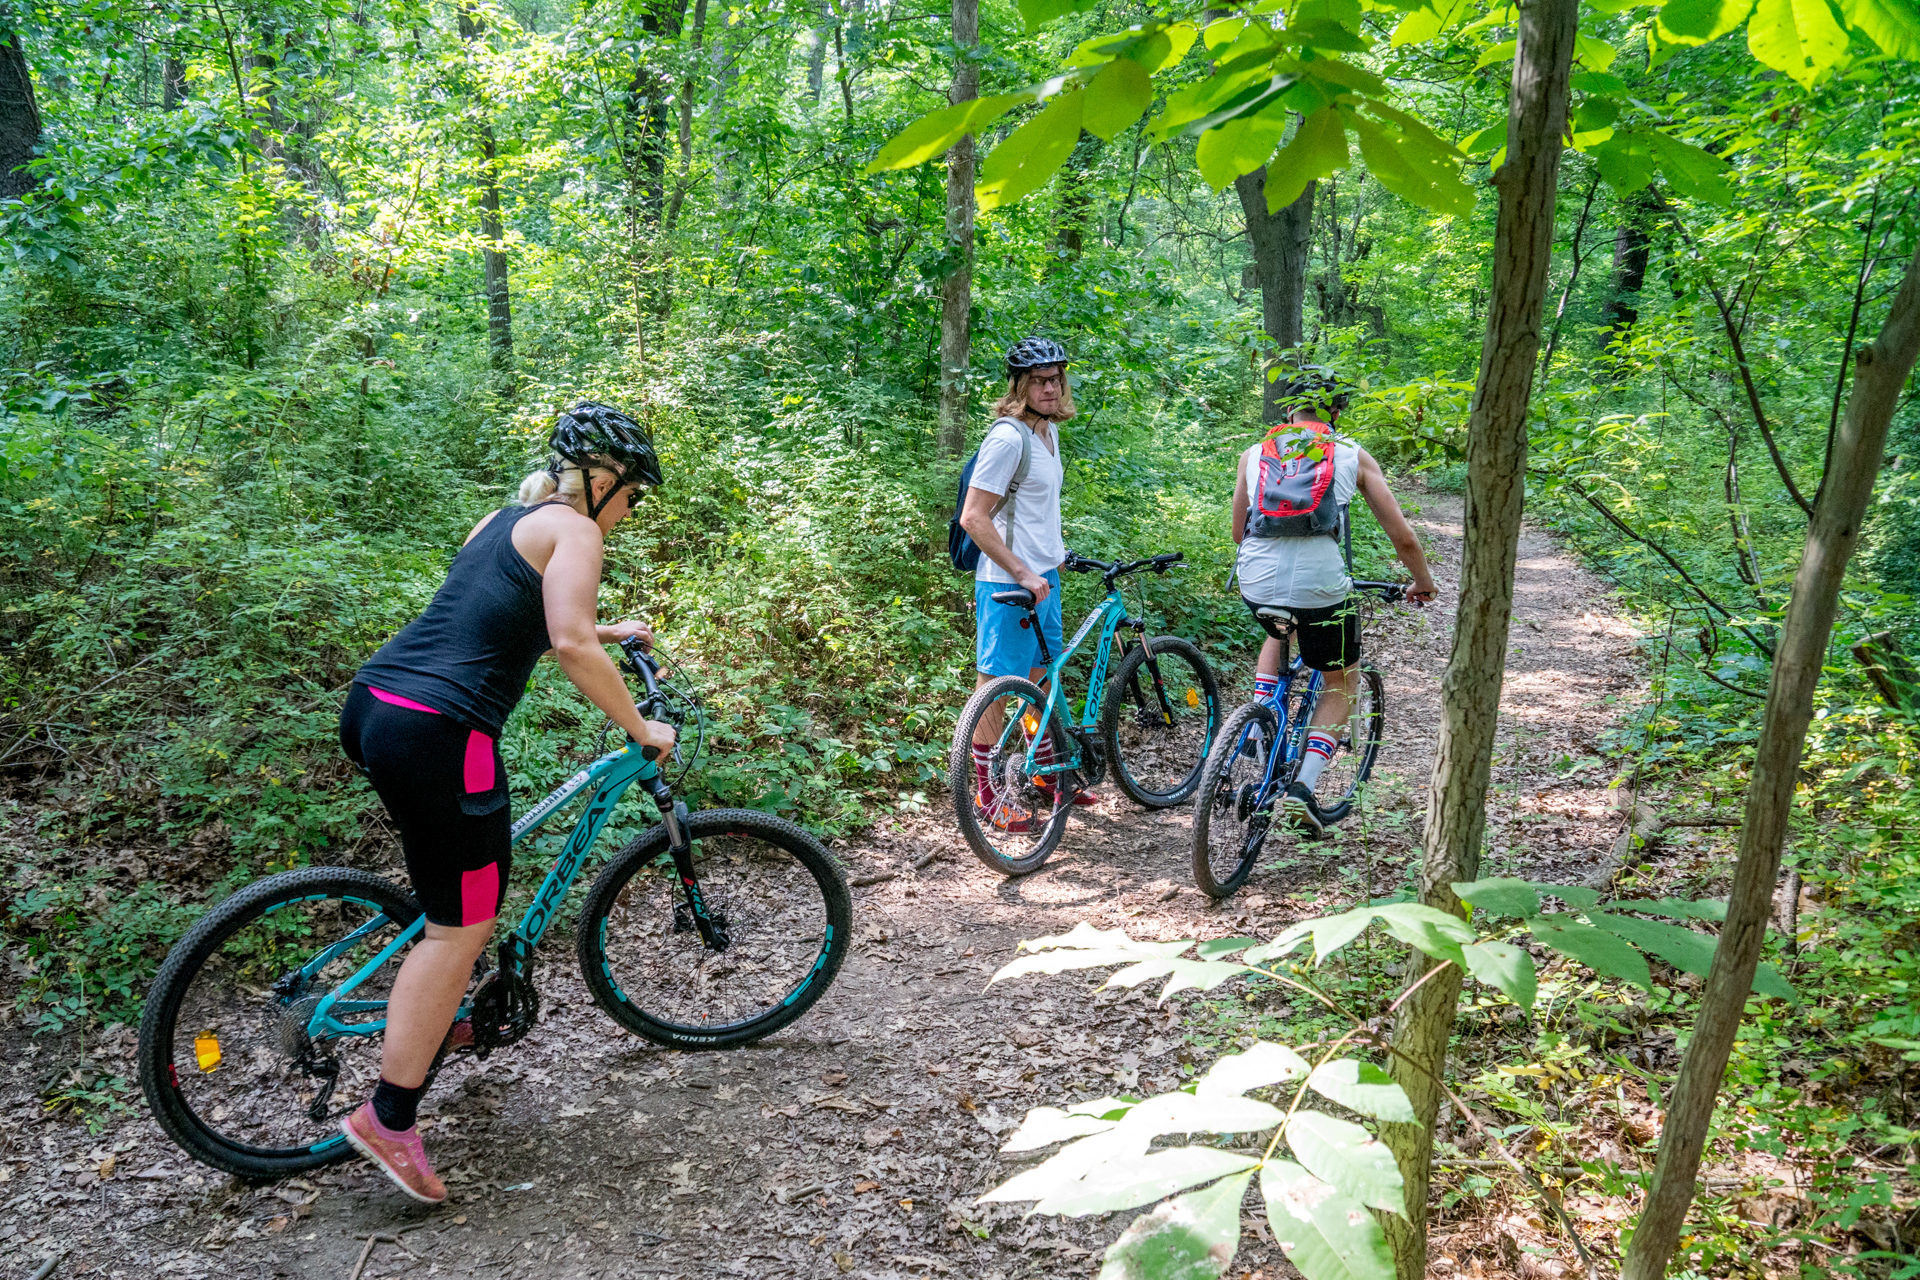
\includegraphics[width=0.75\textwidth]{CunninghamTrails.jpg}
\end{figure}

\begin{figure}[p]
  \caption{``Rock Garden'' Technical Mountain Biking Obstacle}
  \label{RockG}
  \centering
  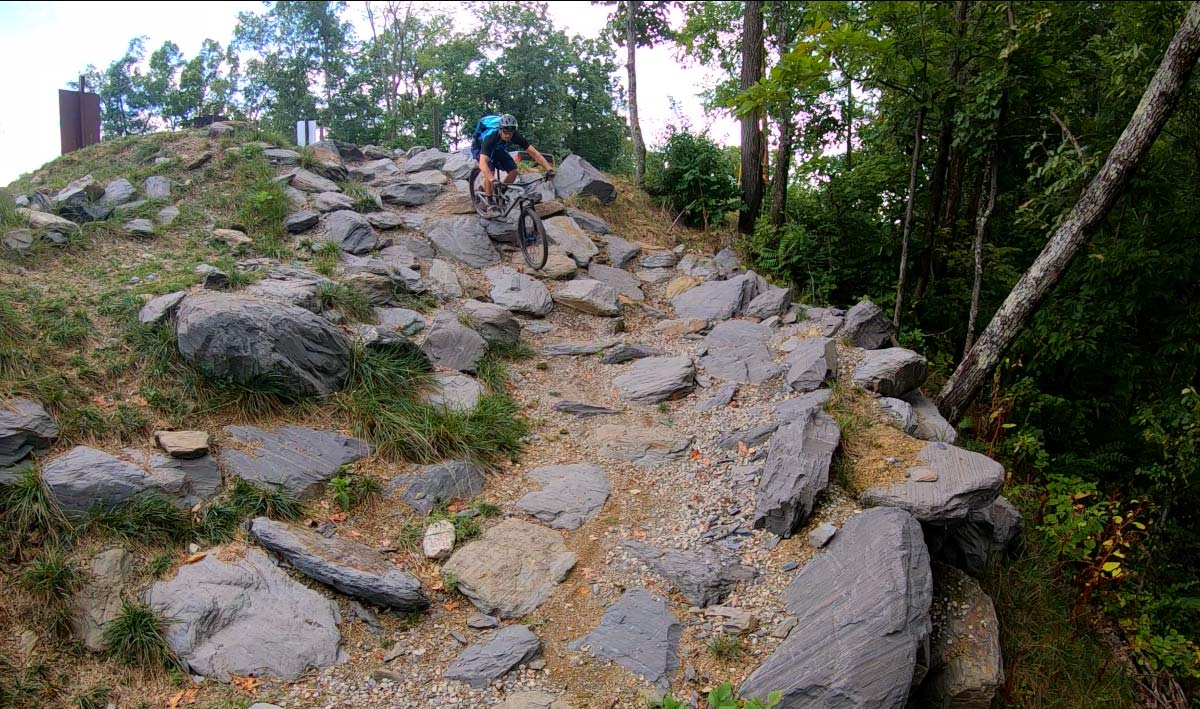
\includegraphics[width=0.75\textwidth]{RockGarden.jpg}
\end{figure}




\end{document}